%% LyX 2.4.0-alpha3 created this file.  For more info, see https://www.lyx.org/.
%% Do not edit unless you really know what you are doing.
\documentclass[UTF8]{ctexrep}
\usepackage[T1]{fontenc}
\setcounter{secnumdepth}{3}
\setcounter{tocdepth}{3}
\usepackage{amsmath}
\usepackage{graphicx}

\makeatletter

%%%%%%%%%%%%%%%%%%%%%%%%%%%%%% LyX specific LaTeX commands.
\newcommand{\lyxmathsym}[1]{\ifmmode\begingroup\def\b@ld{bold}
  \text{\ifx\math@version\b@ld\bfseries\fi#1}\endgroup\else#1\fi}

%% Because html converters don't know tabularnewline
\providecommand{\tabularnewline}{\\}

%%%%%%%%%%%%%%%%%%%%%%%%%%%%%% User specified LaTeX commands.
% 如果没有这一句命令,XeTeX会出错,原因参见
% http://bbs.ctex.org/viewthread.php?tid=60547
\DeclareRobustCommand\nobreakspace{\leavevmode\nobreak\ }

\usepackage{color}
\usepackage{listings}
\lstset{ %
language=Python,                % choose the language of the code
basicstyle=\footnotesize,       % the size of the fonts that are used for the code
numbers=left,                   % where to put the line-numbers
numberstyle=\footnotesize,      % the size of the fonts that are used for the line-numbers
stepnumber=1,                   % the step between two line-numbers. If it is 1 each line will be numbered
numbersep=5pt,                  % how far the line-numbers are from the code
backgroundcolor=\color{white},  % choose the background color. You must add \usepackage{color}
showspaces=false,               % show spaces adding particular underscores
showstringspaces=false,         % underline spaces within strings
showtabs=false,                 % show tabs within strings adding particular underscores
frame=single,           % adds a frame around the code
tabsize=4,          % sets default tabsize to 2 spaces
captionpos=b,           % sets the caption-position to bottom
breaklines=true,        % sets automatic line breaking
breakatwhitespace=false,    % sets if automatic breaks should only happen at whitespace
escapeinside={\%*}{*)}          % if you want to add a comment within your code
}
%\lstset{     
%basicstyle=\tt,        
%showstringspaces=false, 
%} 
%\begin{lstlisting}[language=C]       
%#include <stdio.h> {     
%//Example     
%printf("Hello World");     
%int i, sum = 0;     
%for (i = 0; i < 10; i++){
%        sum += i;     
%}     
%printf("%d", sum);     
%return 0; } 
%\end{lstlisting}
\usepackage{hyperref}
\usepackage{xeCJK}
\setmainfont{MI Lan Pro VF Regular} 
\setCJKmainfont{MI Lan Pro VF Regular}[BoldFont={MI Lan Pro VF Bold}, ItalicFont={MI Lan Pro VF Light}]
\usepackage[UTF8,nofonts]{ctexcap}

\makeatother

\begin{document}
\title{深度学习简单教程}
\author{秦以南}
\maketitle
\begin{abstract}
这个教程是由我在学习Deep Learning的过程中写成的,现在分享给大家,希望大家可以更好的理解它\textasciitilde{}
\end{abstract}
\tableofcontents{}

\chapter{机器学习和深度学习综述}

\section{人工智能、机器学习、深度学习的关系}

近些年人工智能、机器学习和深度学习的概念十分火热,但很多从业者却很难说清它们之间的关系,外行人更是雾里看花。在研究深度学习之前,先从三个概念的正本清源开始。概括来说,人工智能、机器学习和深度学习覆盖的技术范畴是逐层递减的,三者的关系如图\ref{fig:1.1}所示,即:人工智能
> 机器学习 > 深度学习。
\begin{center}
\begin{figure}
\begin{centering}
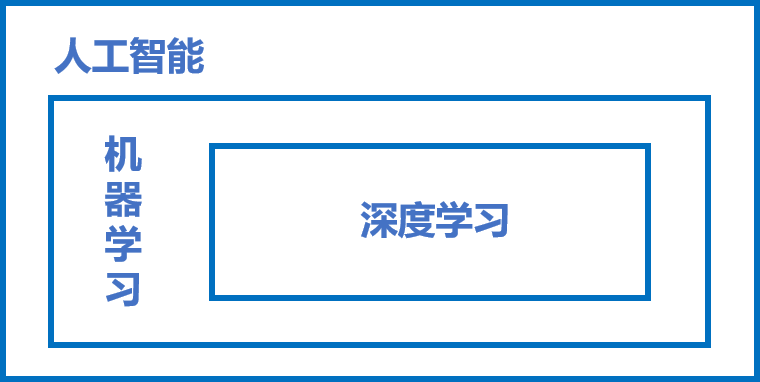
\includegraphics[scale=0.5]{imgs/chapter1/1}
\par\end{centering}
\caption{人工智能、机器学习和深度学习三者关系示意\protect\label{fig:1.1}}
\end{figure}
\par\end{center}

人工智能(ArtificialIntelligence,AI)是最宽泛的概念,是研发用于模拟、延伸和扩展人的智能的理论、方法、技术及应用系统的一门新的技术科学。由于这个定义只阐述了目标,而没有限定方法,因此实现人工智能存在的诸多方法和分支,导致其变成一个“大杂烩”式的学科。机器学习(MachineLearning,ML)是当前比较有效的一种实现人工智能的方式。深度学习(DeepLearning,DL)是机器学习算法中最热门的一个分支,近些年取得了显著的进展,并替代了大多数传统机器学习算法。

\section{机器学习}

区别于人工智能,机器学习、尤其是监督学习则有更加明确的指代。机器学习是专门研究计算机怎样模拟或实现人类的学习行为,以获取新的知识或技能,重新组织已有的知识结构,使之不断改善自身的性能。这句话有点“云山雾罩”的感觉,让人不知所云,下面我们从机器学习的实现和方法论两个维度进行剖析,帮助读者更加清晰地认识机器学习的来龙去脉。

\subsection{机器学习的实现}

机器学习的实现可以分成两步:训练和预测,类似于归纳和演绎:
\begin{itemize}
\item 归纳: 从具体案例中抽象一般规律,机器学习中的“训练”亦是如此。从一定数量的样本(已知模型输入$X$和模型输出$Y$)中,学习输出$\bar{{Y}}$与输入$\bar{{X}}$的关系(可以想象成是某种表达式)。
\item 演绎: 从一般规律推导出具体案例的结果,机器学习中的“预测”亦是如此。基于训练得到的$Y$与$X$之间的关系,如出现新的输入$X$,计算出输出$Y$。通常情况下,如果通过模型计算的输出和真实场景的输出一致,则说明模型是有效的。
\end{itemize}

\subsection{机器学习的方法论}

机器学习的方法论和人类科研的过程有着异曲同工之妙,下面以“机器从牛顿第二定律实验中学习知识”为例,帮助读者更加深入理解机器学习(监督学习)的方法论本质,即在“机器思考”的过程中确定模型的三个关键要素:假设、评价、优化。

\subsubsection{案例:机器从牛顿第二定律实验中学习知识}

\paragraph{牛顿第二定律}

牛顿第二定律是艾萨克·牛顿在1687年于《自然哲学的数学原理》一书中提出的,其常见表述:物体加速度的大小跟作用力成正比,跟物体的质量成反比,与物体质量的倒数成正比。牛顿第二运动定律和第一、第三定律共同组成了牛顿运动定律,阐述了经典力学中基本的运动规律。

在中学课本中,牛顿第二定律有两种实验设计方法:倾斜滑动法和水平拉线法,如图\ref{fig:1.2}所示。
\begin{center}
\begin{figure}
\centering{}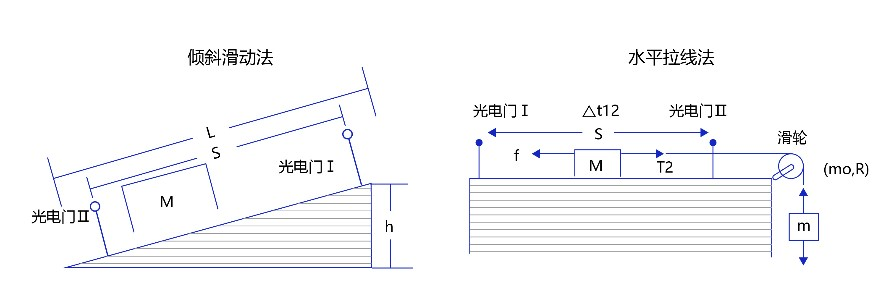
\includegraphics[scale=0.5]{imgs/chapter1/2}\caption{牛顿第二定律实验设计方法\protect\label{fig:1.2}}
\end{figure}
\par\end{center}

通过多次实验数据,可以统计出如表\ref{tab:1.1}所示的不同作用力下的木块加速度。
\begin{center}
\begin{table}
\begin{centering}
\begin{tabular}{ccc}
\hline 
项目 & 作用力$X$ & 加速度$Y$\tabularnewline
\hline 
第1次 & 4 & 2\tabularnewline
第2次 & 4 & 2\tabularnewline
$\cdots$ & $\cdots$ & $\cdots$\tabularnewline
第n次 & 6 & 3\tabularnewline
\hline 
\end{tabular}
\par\end{centering}
\caption{实验获取的大量数据样本和观测结果\protect\label{tab:1.1}}
\end{table}
\par\end{center}

观察实验数据不难猜测,物体的加速度$a$和作用力$F$之间的关系应该是线性关系。因此我们提出假设 $a=w\cdot F$,其中,$a$代表加速度,$F$代表作用力,$w$是待确定的参数。

通过大量实验数据的训练,确定参数$w$是物体质量的倒数$(1/m)$,即得到完整的模型公式$a=F\cdot(1/m)$。当已知作用到某个物体的力时,基于模型可以快速预测物体的加速度。例如:燃料对火箭的推力$F=10$,火箭的质量$m=2$,可快速得出火箭的加速度$a=5$。

\subsubsection{如何确定模型参数?}

这个有趣的案例演示了机器学习的基本过程,但其中有一个关键点的实现尚不清晰,即:\textbf{如何确定模型参数}$\lyxmathsym{(}w=1/m\lyxmathsym{)}$?

确定参数的过程与科学家提出假说的方式类似,合理的假说可以最大化的解释所有的已知观测数据。如果未来观测到不符合理论假说的新数据,科学家会尝试提出新的假说。如:天文史上,使用大圆和小圆组合的方式计算天体运行,在中世纪是可以拟合观测数据的。但随着欧洲工业革命的推动,天文观测设备逐渐强大,已有的理论已经无法解释越来越多的观测数据,这促进了使用椭圆计算天体运行的理论假说出现。因此,\textbf{模型有效的基本条件是能够拟合已知的样本},这给我们提供了学习有效模型的实现方案。

图\ref{fig:1.3}是以$H$为模型的假设,它是一个关于参数$w$和输入$x$的函数,用$H(w,x)$表示。模型的优化目标是$H(w,x)$的输出与真实输出$Y$尽量一致,两者的相差程度即是模型效果的评价函数(相差越小越好)。那么,确定参数的过程就是在已知的样本上,不断减小该评价函数($H$和$Y$的差距)的过程。直到模型学习到一个参数$w$,使得评价函数的值最小,\textbf{衡量模型预测值和真实值差距的评价函数也被称为损失函数(损失Loss)}。
\begin{center}
\begin{figure}
\begin{centering}
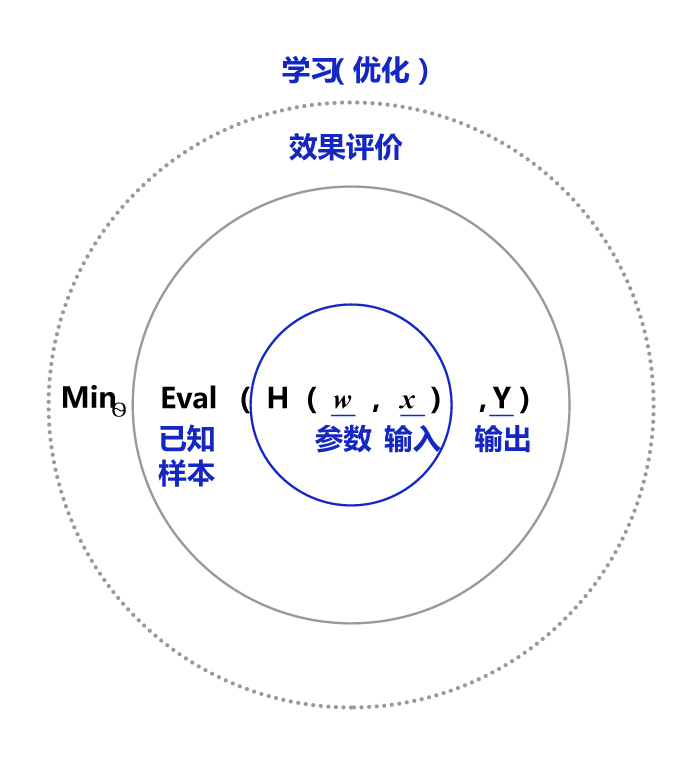
\includegraphics[scale=0.25]{imgs/chapter1/3}
\par\end{centering}
\caption{确定模型参数示意图\protect\label{fig:1.3}}
\end{figure}
\par\end{center}

假设机器通过尝试答对(最小化损失)大量的习题(已知样本)来学习知识(模型参数$w$),并期望用学习到的知识所代表的模型$H(w,x)$,回答不知道答案的考试题(未知样本)。最小化损失是模型的优化目标,实现损失最小化的方法称为优化算法,也称为寻解算法(找到使得损失函数最小的参数解)。参数$w$和输入$x$组成公式的基本结构称为假设。在牛顿第二定律的案例中,基于对数据的观测,我们提出了线性假设,即作用力和加速度是线性关系,用线性方程表示。由此可见,\textbf{模型假设、评价函数(损失/优化目标)和优化算法是构成模型的三个关键要素}。

\subsubsection{模型结构}

模型假设、评价函数和优化算法是如何支撑机器学习流程的呢?如图\ref{fig:1.4} 所示。
\begin{center}
\begin{figure}

\begin{centering}
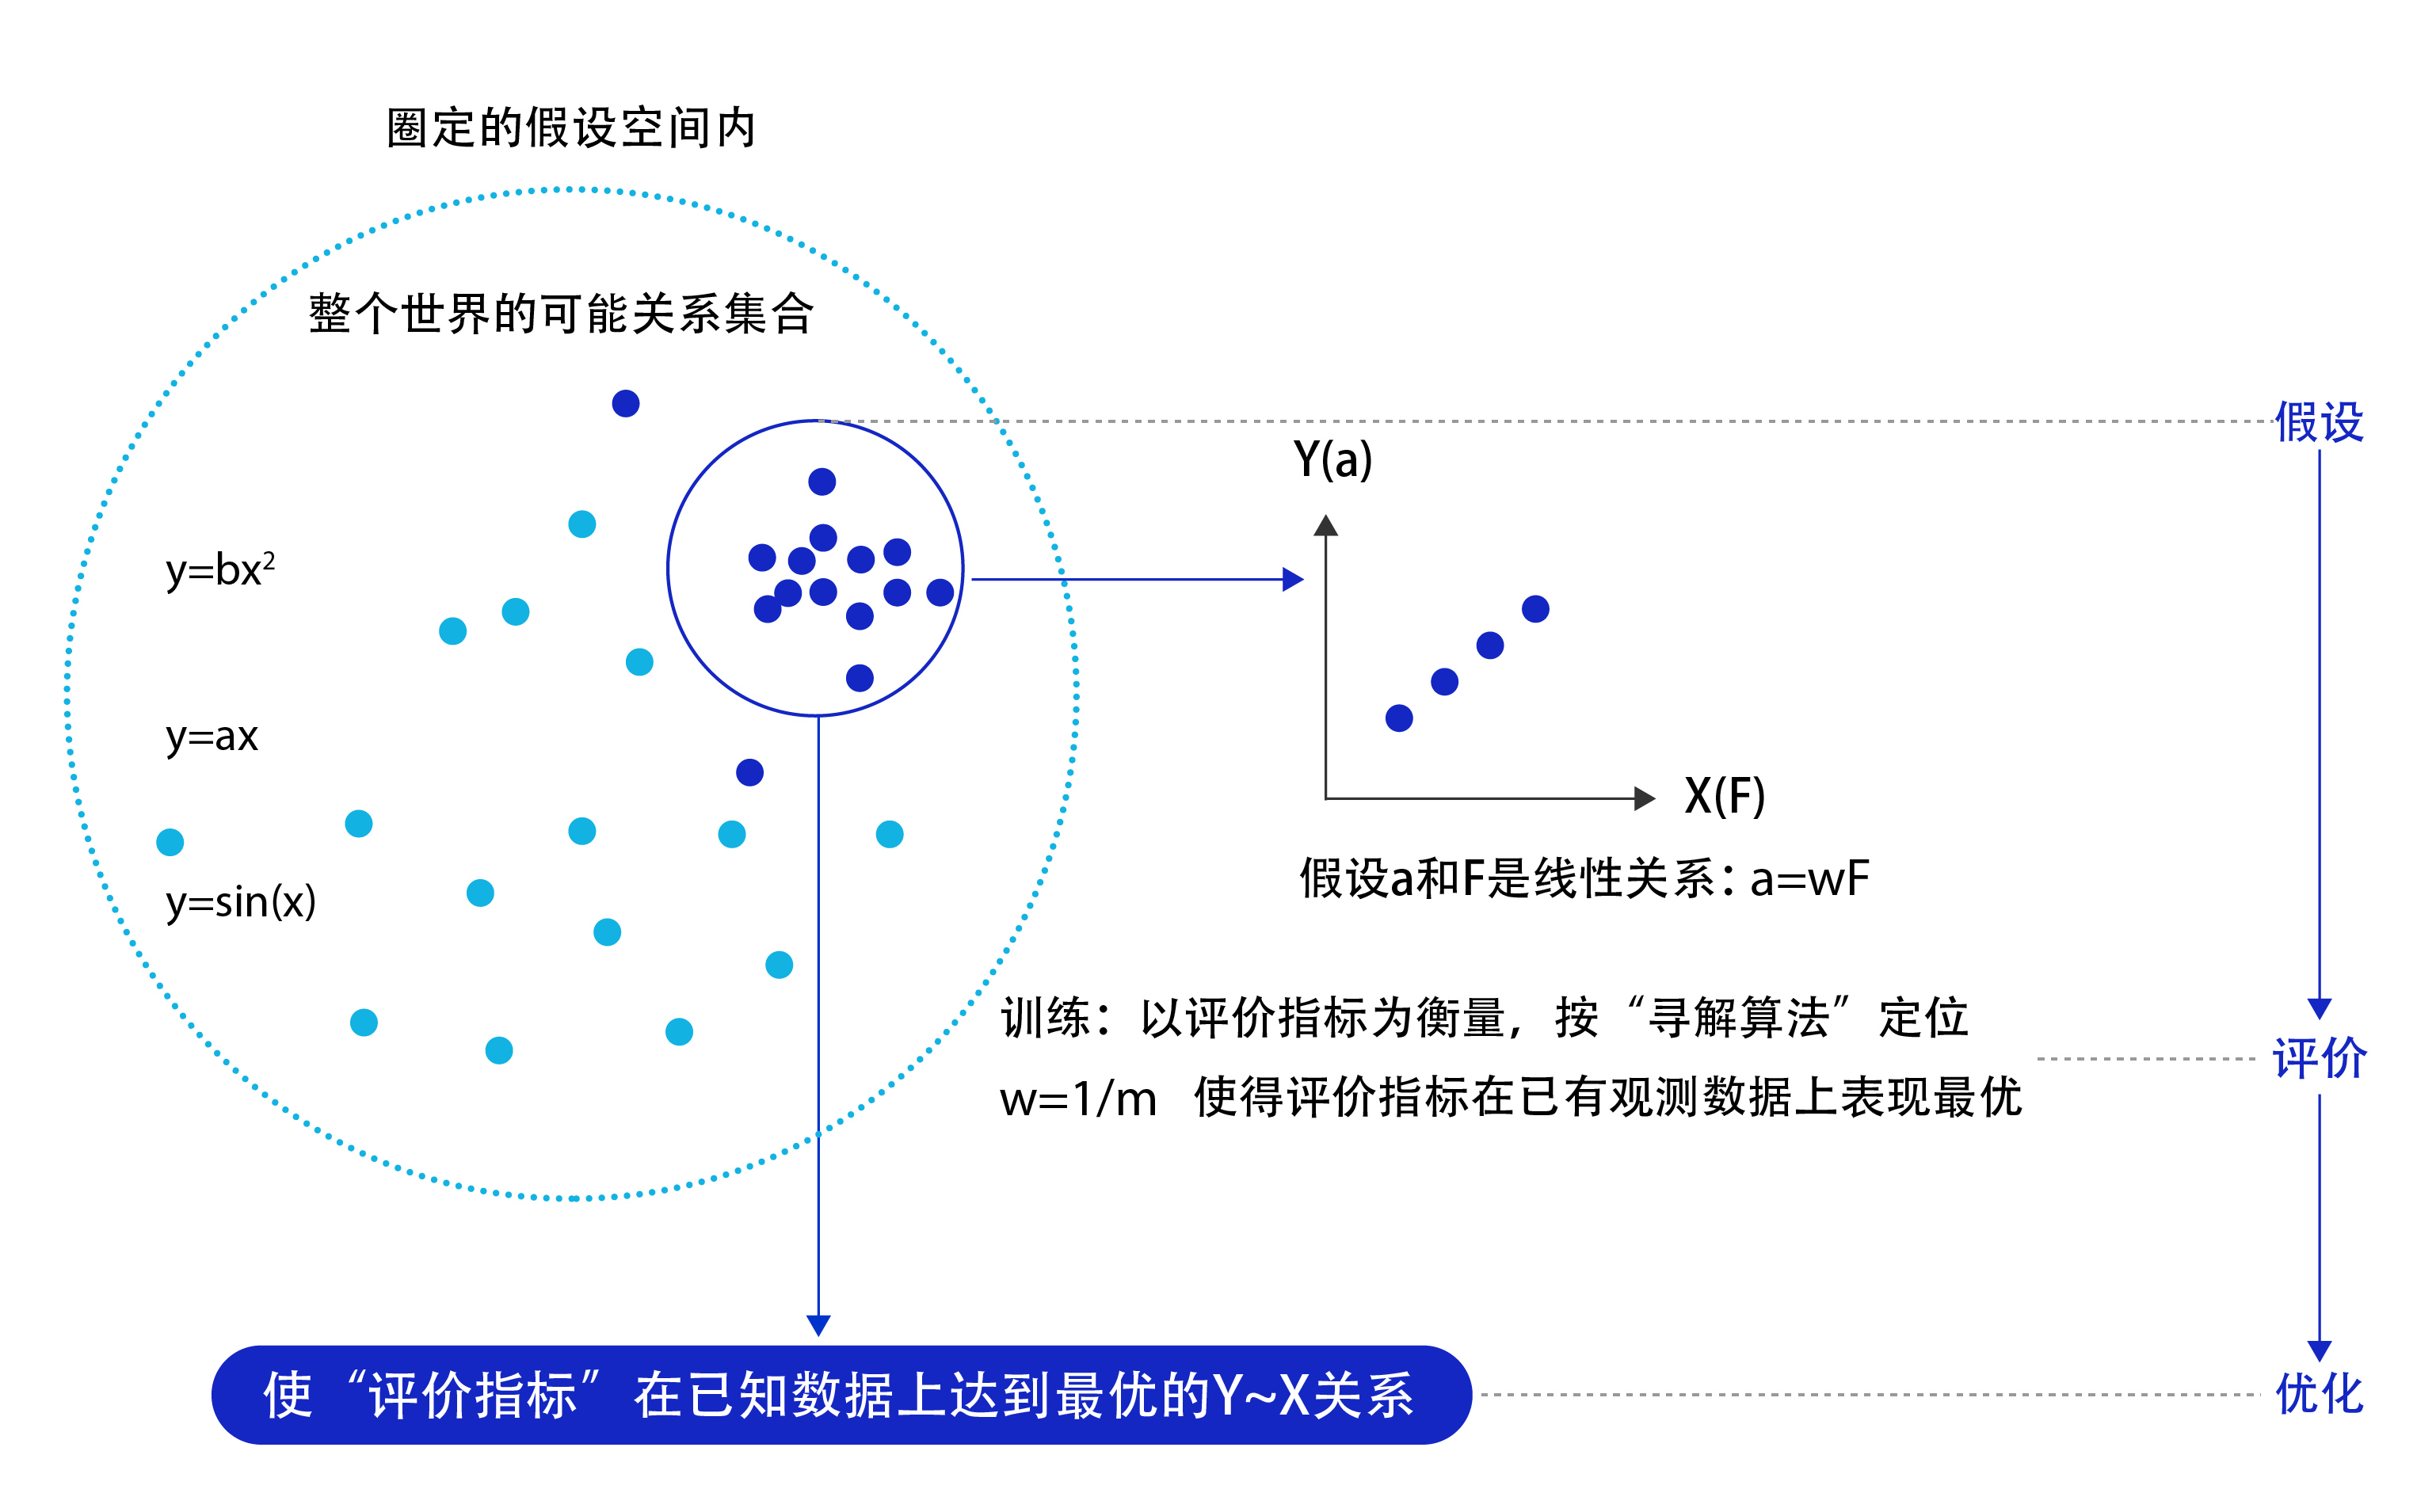
\includegraphics[scale=0.45]{imgs/chapter1/4}
\par\end{centering}
\caption{机器学习流程\protect\label{fig:1.4}}

\end{figure}
\par\end{center}
\begin{itemize}
\item \textbf{模型假设}:世界上的可能关系千千万,漫无目标的试探$Y\sim X$之间的关系显然是十分低效的。因此假设空间先圈定了一个模型能够表达的关系可能,如蓝色圆圈所示。机器还会进一步在假设圈定的圆圈内寻找最优的$Y\sim X$关系,即确定参数$w$。
\item \textbf{评价函数}:寻找最优之前,我们需要先定义什么是最优,即评价一个$Y\sim X$关系的好坏的指标。通常衡量该关系是否能很好的拟合现有观测样本,将拟合的误差最小作为优化目标。
\item \textbf{优化算法}:设置了评价指标后,就可以在假设圈定的范围内,将使得评价指标最优(损失函数最小/最拟合已有观测样本)的$Y\sim X$关系找出来,这个寻找最优解的方法即为优化算法。最笨的优化算法即按照参数的可能,穷举每一个可能取值来计算损失函数,保留使得损失函数最小的参数作为最终结果。
\end{itemize}
从上述过程可以得出,机器学习的过程与牛顿第二定律的学习过程基本一致,都分为假设、评价和优化三个阶段:
\begin{enumerate}
\item \textbf{假设}:通过观察加速度$a$和作用力$F$的观测数据,假设$a$和$F$是线性关系,即$a=w\cdot F$。
\item \textbf{评价}:对已知观测数据上的拟合效果好,即$w\cdot F$计算的结果要和观测的$a$尽量接近。
\item \textbf{优化}:在参数$w$的所有可能取值中,发现$w=1/m$可使得评价最好(最拟合观测样本)。
\end{enumerate}
机器执行学习任务的框架体现了其\textbf{学习的本质是“参数估计”}(Learning is parameter estimation)。

上述方法论使用更规范化的表示如图\ref{fig:1.5}所示,未知目标函数$f$,以训练样本${D}=\lyxmathsym{(}{x_{1}}\lyxmathsym{,}{y_{1}}\lyxmathsym{),}\ldots\lyxmathsym{,(}{x_{n}}\lyxmathsym{,}{y_{n}}$)为依据。从假设集合$H$中,通过学习算法$A$找到一个函数$g$。如果$g$能够最大程度的拟合训练样本$D$,那么可以认为函数$g$就接近于目标函数$f$。
\begin{center}
\begin{figure}
\begin{centering}
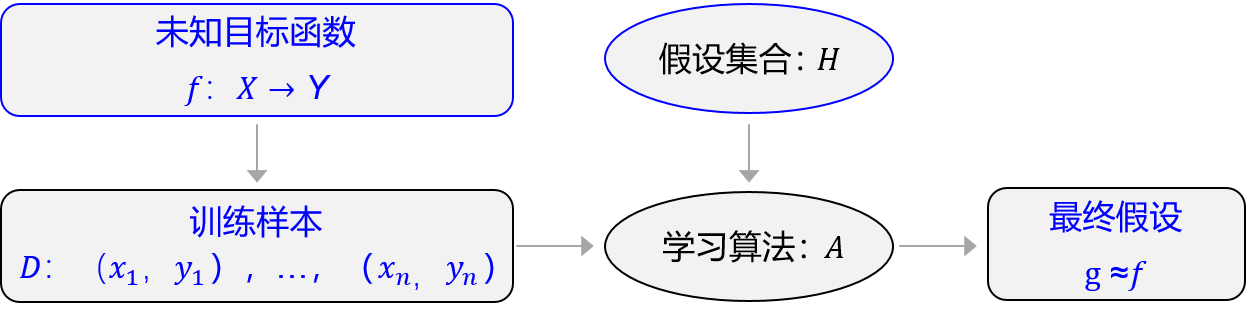
\includegraphics[scale=0.5]{imgs/chapter1/5}
\par\end{centering}
\caption{规范化表示\protect\label{fig:1.5}}

\end{figure}
\par\end{center}

在此基础上,许多看起来完全不一样的问题都可以使用同样的框架进行学习,如科学定律、图像识别、机器翻译和自动问答等,它们的学习目标都是拟合一个“大公式f”,如
图\ref{fig:1.6} 所示。
\begin{center}
\begin{figure}
\begin{centering}
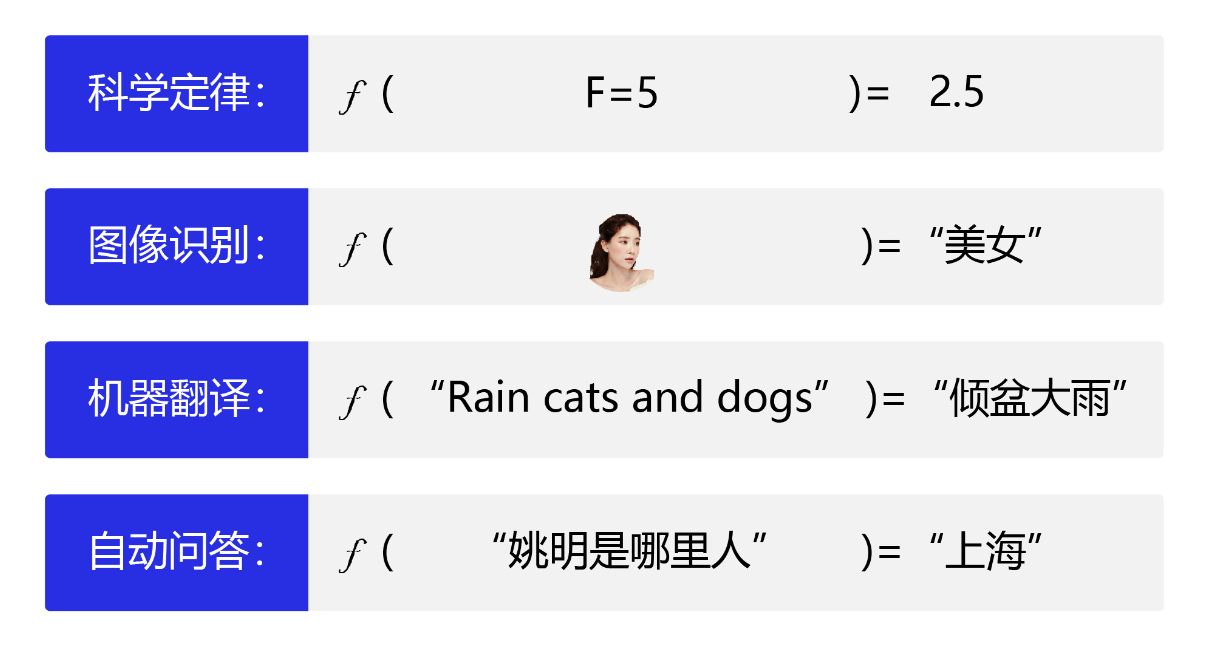
\includegraphics[scale=0.35]{imgs/chapter1/6}
\par\end{centering}
\caption{机器学习就是拟合一个“大公式” \protect\label{fig:1.6}}
\end{figure}
\par\end{center}

\section{深度学习}

机器学习算法理论在上个世纪90年代发展成熟,在许多领域都取得了成功,但平静的日子只延续到2010年左右。随着大数据的涌现和计算机算力提升,深度学习模型异军突起,极大改变了机器学习的应用格局。今天,多数机器学习任务都可以使用深度学习模型解决,尤其在语音、计算机视觉和自然语言处理等领域,深度学习模型的效果比传统机器学习算法有显著提升。

相比传统的机器学习算法,深度学习做出了哪些改进呢?其实\textbf{两者在理论结构上是一致的,即:模型假设、评价函数和优化算法,其根本差别在于假设的复杂度}。如
图\ref{fig:1.6} 第二个示例(图像识别)所示,对于美女照片,人脑可以接收到五颜六色的光学信号,能快速反应出这张图片是一位美女,而且是程序员喜欢的类型。但对计算机而言,只能接收到一个数字矩阵,对于美女这种高级的语义概念,从像素到高级语义概念中间要经历的信息变换的复杂性是难以想象的,如图\ref{fig:1.7}所示。
\begin{center}
\begin{figure}
\begin{centering}
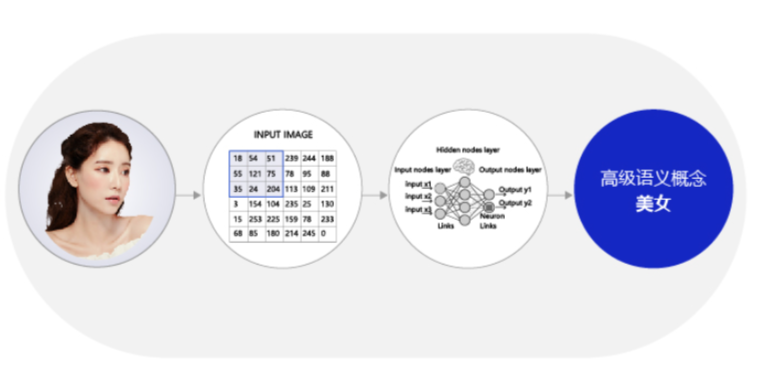
\includegraphics[scale=0.6]{imgs/chapter1/7}
\par\end{centering}
\caption{深度学习的模型复杂度难以想象\protect\label{fig:1.7}}

\end{figure}
\par\end{center}

这种变换已经无法用数学公式表达,因此研究者们借鉴了人脑神经元的结构,设计出神经网络的模型,如图\ref{fig:1.8}所示。图\ref{fig:1.8}(a)展示了神经网络基本单元-感知机的设计方案,其处理信息的方式与人脑中的单一神经元有很强的相似性;图\ref{fig:1.8}(b)展示了几种经典的神经网络结构(后续的章节中会详细阐述),类似于人脑中多种基于大量神经元连接而形成的不同职能的器官。
\begin{center}
\begin{figure}
\begin{centering}
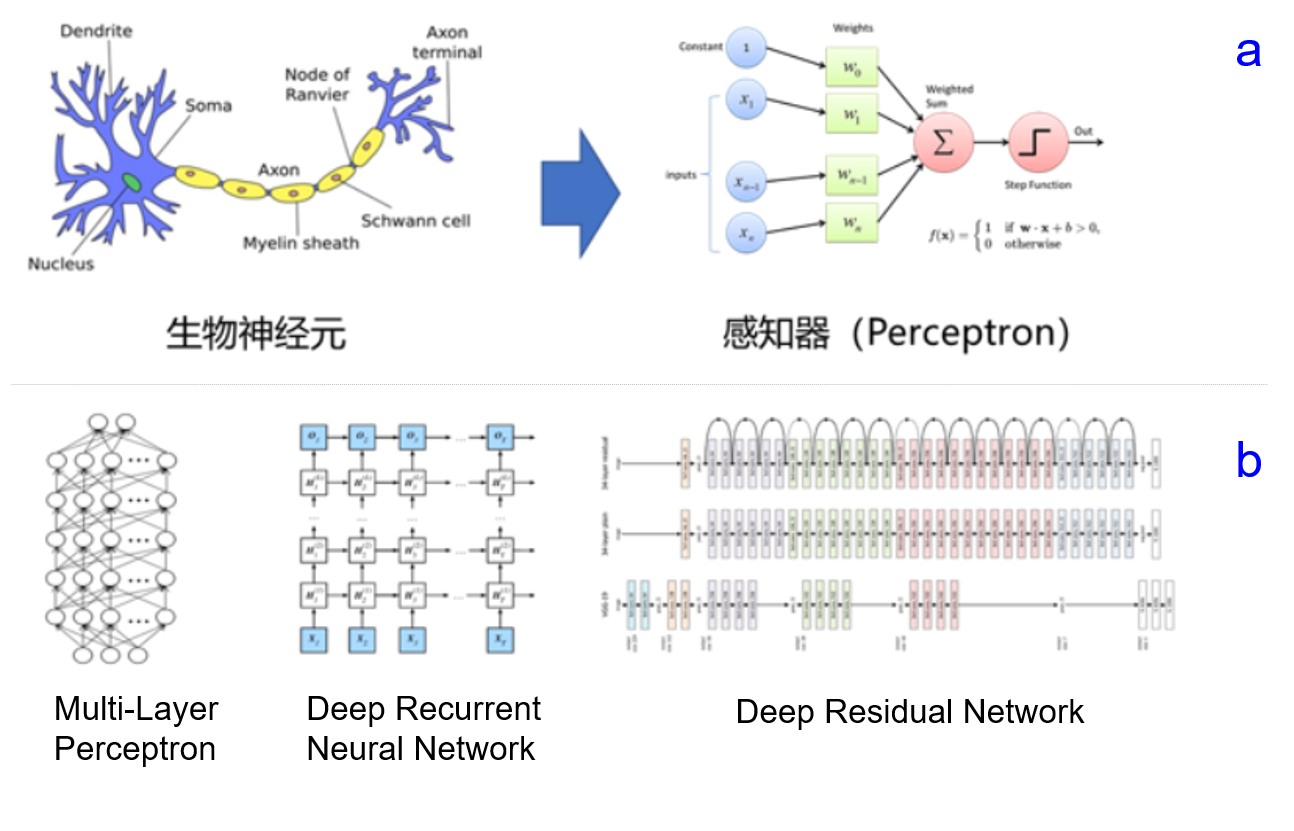
\includegraphics[scale=0.5]{imgs/chapter1/8}
\par\end{centering}
\caption{模拟人脑结构,针对各种任务设计不同的深度学习模型\protect\label{fig:1.8}}
\end{figure}
\par\end{center}

\subsection{神经网络的基本概念}

人工神经网络包括多个神经网络层,如:卷积层、全连接层、LSTM等,每一层又包括很多神经元,超过三层的非线性神经网络都可以被称为深度神经网络。通俗的讲,深度学习的模型可以视为是输入到输出的映射函数,如图像到高级语义(美女)的映射,足够深的神经网络理论上可以拟合任何复杂的函数。因此神经网络非常适合学习样本数据的内在规律和表示层次,对文字、图像和语音任务有很好的适用性。这几个领域的任务是人工智能的基础模块,因此深度学习被称为实现人工智能的基础也就不足为奇了。

神经网络基本结构如 图\ref{fig:1.9} 所示。

\begin{figure}
\begin{centering}
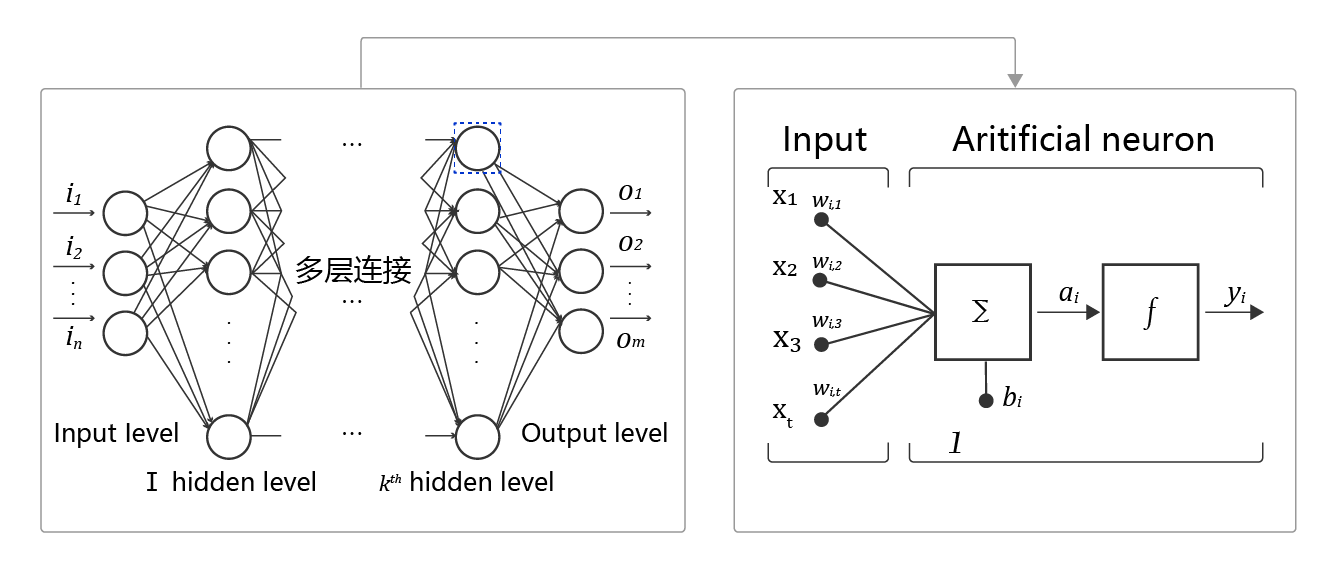
\includegraphics[scale=0.5]{imgs/chapter1/9}
\par\end{centering}
\caption{神经网络基本结构示意图\protect\label{fig:1.9}}
\end{figure}

\begin{itemize}
\item 神经元: 神经网络中每个节点称为神经元,由两部分组成:
\begin{itemize}
\item 加权和:将所有输入加权求和。
\item 非线性变换(激活函数):加权和的结果经过一个非线性函数变换,让神经元计算具备非线性的能力。
\end{itemize}
\item 多层连接: 大量这样的节点按照不同的层次排布,形成多层的结构连接起来,即称为神经网络。
\item 前向计算: 从输入计算输出的过程,顺序从网络前至后。
\item 计算图: 以图形化的方式展现神经网络的计算逻辑又称为计算图,也可以将神经网络的计算图以公式的方式表达:
\end{itemize}
\begin{center}
$Y=f_{3}(f_{2}(f_{1}(w_{1}\cdot x_{1}+w_{2}\cdot x_{2}+w_{3}\cdot x_{3}+b)+\ldots)\ldots)\ldots)$
\par\end{center}

由此可见,神经网络并没有那么神秘,它的本质是一个含有很多参数的“大公式”。

\subsection{深度学习的发展历程}

神经网络思想的提出已经是70多年前的事情了,现今的神经网络和深度学习的设计理论是一步步趋于完善的。在这漫长的发展岁月中,一些取得关键突破的闪光时刻,值得深度学习爱好者们铭记,如
图\ref{fig:1.10} 所示。
\begin{center}
\begin{figure}
\begin{centering}
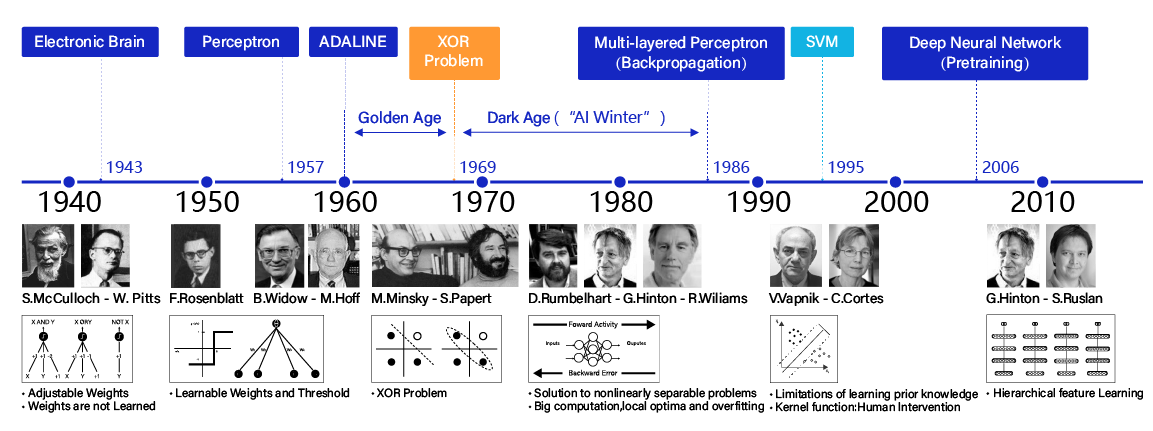
\includegraphics[scale=0.28]{imgs/chapter1/10}
\par\end{centering}
\caption{深度学习发展历程\protect\label{fig:1.10}}
\end{figure}
\par\end{center}
\begin{itemize}
\item \textbf{1940年代}:首次提出神经元的结构,但权重是不可学的。
\item \textbf{50-60年代}:提出权重学习理论,神经元结构趋于完善,开启了神经网络的第一个黄金时代。
\item \textbf{1969年}:提出异或问题(人们惊讶的发现神经网络模型连简单的异或问题也无法解决,对其的期望从云端跌落到谷底),神经网络模型进入了被束之高阁的黑暗时代。
\item \textbf{1986年}:新提出的多层神经网络解决了异或问题,但随着90年代后理论更完备并且实践效果更好的SVM等机器学习模型的兴起,神经网络并未得到重视。
\item \textbf{2010年左右}:深度学习进入真正兴起时期。随着神经网络模型改进的技术在语音和计算机视觉任务上大放异彩,也逐渐被证明在更多的任务,如自然语言处理以及海量数据的任务上更加有效。至此,神经网络模型重新焕发生机,并有了一个更加响亮的名字:深度学习。
\end{itemize}
为何神经网络到2010年后才焕发生机呢?这与深度学习成功所依赖的先决条件:大数据涌现、硬件发展和算法优化有关。
\begin{itemize}
\item \textbf{大数据是神经网络发展的有效前提}。神经网络和深度学习是非常强大的模型,需要足够量级的训练数据。时至今日,之所以很多传统机器学习算法和人工特征依然是足够有效的方案,原因在于很多场景下没有足够的标记数据来支撑深度学习。深度学习的能力特别像科学家阿基米德的豪言壮语:“给我一根足够长的杠杆,我能撬动地球!”。深度学习也可以发出类似的豪言:“给我足够多的数据,我能够学习任何复杂的关系”。但在现实中,足够长的杠杆与足够多的数据一样,往往只能是一种美好的愿景。直到近些年,各行业IT化程度提高,累积的数据量爆发式地增长,才使得应用深度学习模型成为可能。
\item \textbf{依靠硬件的发展和算法的优化}。现阶段,依靠更强大的计算机、GPU、autoencoder预训练和并行计算等技术,深度学习在模型训练上的困难已经被逐渐克服。其中,数据量和硬件是更主要的原因。没有前两者,科学家们想优化算法都无从进行。
\end{itemize}

\section{小结}

虽然历史悠久,但深度学习在今天依然在蓬勃发展,一方面基础研究快速发展,另一方面工业实践层出不穷。基于深度学习的顶级会议ICLR(International
Conference on Learning Representations)统计,深度学习相关的论文数量呈逐年递增的状态。同时,不仅仅是深度学习会议,与数据和模型技术相关的会议ICML和KDD,专注视觉的CVPR和专注自然语言处理的EMNLP等国际会议的大量论文均涉及着深度学习技术。该领域和相关领域的研究方兴未艾,技术仍在不断创新突破中。

另一方面,以深度学习为基础的人工智能技术,在升级改造众多的传统行业领域,存在极其广阔的应用场景。人工智能技术不仅可在众多行业中落地应用(广度),同时,在部分行业(如安防、遥感、互联网、金融、工业等)已经实现了市场化变现和高速增长(深度),为社会贡献了巨大的经济价值。

\chapter{深度学习概念简介}

\section{机器学习基本概念}

由于深度学习是一种特殊的机器学习方法,一般的机器学习概念对于深度学习也适用。为了能够更好地对深度学习的一些概念做阐述,这里把机器学习的概念作
为独立的一节,希望能够帮助读者更好地理解深度学习的基本概念。

\subsection{机器学习的主要任务}

首先让我们了解一下机器学习的主要任务。一般来说,我们可以把这个任务描述为:给定在现实中获取的一系列\textbf{数据}来构建一个\textbf{模型},用于描述数据的具体\textbf{分布}(这个分布指的是概率论意义上的分布。也就是说,某些数据可能出现得比较频繁,另外一些数据可能出现得比较稀少,我们需要描述什么数据比较可能出现,并且用概率来描述数据出现的可能性)。在这里用粗体标出了三个重要的词,下面详细介绍一下这些词的具体意义。

\textbf{数据}是人们对周围发生的一些现象的数字化描述。我们在现实中获取的数据是各种各样的,比如图片(计算机使用像素的排列来表示图片,其中每个像素可表示为三个数值(即红绿蓝(RGB))或四个数值和透明度(RGBA))、文本(计算机使用字符串来表示文本)、音频(计算机中一个比较通用的格式是使用16bit(即65536个值)来代表声音的振幅,按照一定采样频率如44.1kHz来组成一段音频。)等。

这些数据可以分成有标签的(比如电影评论的文本和文本对应的评价)和没有标签的(比如只是一段文本)。根据能够处理的数据类型,机器学习的任务大致可以分为两类:监督学习(Supervised
Learning)和无监督学习(Unsupervised Learning)。前者指的是,我们拥有具体的数据和预测目标(标签),需要从数据出发构造具体的模型预测这些目标,当然模型预测越准确越好,其代表的主要任务包括回归(预测连续的值,如根据历史的气温预测未来的气温)和分类(预测离散的值,如根据图片预测图片描述的具体物体的类型)。后者指的是,我们只有数据,没有预测目标,需要构造具体的模型来找出数据的具体规律,其代表的主要任务包括聚类(找出相似的多组数据并把它们归类)。当然,实际上还有介于监督学习和无监督学习方法之间的
半监督学习(Semi-supervised Learning),这里限于篇幅,就不具体展开介绍。

\textbf{模型}是另一个在机器学习中经常碰到的概念。大多数机器学习任务的目的可以归纳为得到一个模型,用这个模型来描述给定的数据。得到这个模型的过程称之为机器学习模型的训练过程。从概率论的角度说,我们可以认为机器学习模型是一个\textbf{概率分布
$P_{\theta}(X)$}(这里以概率密度函数来代表概率分布),其中 $X$ 是训练数据,这个概率分布拥有参数$\boldsymbol{\theta}=\left(\theta_{1},\theta_{2},\cdots,\theta_{n}\right)$(这个参数可以是一个或多个,我们用粗体字母来代表所有的参数
,$n$代表参数的个数)。

机器学习的任务就是求最优参数$\boldsymbol{\theta_{t}}$使得概率分布$\boldsymbol{P_{\theta}(X)}$最大。我们可以用式\ref{eq:2.1}来代表这个过程,其中$argmax$函数代表的是取参数使得数据的概率密度最大。求解最优参数$\boldsymbol{\theta_{t}}$的过程,我们称之为模型的训练过程(Training),用来训练这个模型的数据集称之为\textbf{训练集}(Training
Set),由此得到的模型就可以用来做相应的预测。

\begin{equation}
\boldsymbol{\theta_{t}=}\underset{\theta}{argmax}\,\boldsymbol{P_{\theta}(X)}\label{eq:2.1}
\end{equation}

由于用于机器学习的训练集通常有很多条具体数据,我们可以把训练数据 $\boldsymbol{X}$拆成单条数据的集合,即$\boldsymbol{X=\boldsymbol{(X_{1,}X_{2,}\cdots,X_{n})}}$,其中$n$为数据的总数目,$X$为数据的\textbf{批次}(batch),$X$的子集称之为数据的\textbf{迷你批次}(mini-batch)。假设训练数据的单条数据之间相互独立,我们可以把式\ref{eq:2.1}进一步展开成式\ref{eq:2.2}。需要注意的是,这里把对于独立单条数据的乘积取对数变成了求概率的对数的和,该方法是机器学习推导公式时经常使用的一个方法,我们把整体的求解最优参数$\boldsymbol{\theta_{t}}$的过程称之为\textbf{极大似然估计}(Maximum
LikeIihood Estimation,MLE)。

\begin{equation}
\boldsymbol{\theta_{t}=}\underset{\theta}{argmax}\,\boldsymbol{\underset{i}{\prod}P_{\theta}(X_{i})=\underset{\theta}{argmax}\,\boldsymbol{\underset{i}{\sum}log{P_{\theta}(X_{i})}}}\label{eq:2.2}
\end{equation}


\subsection{机器模型的类型}

以上的机器学习理论适用于所有的机器学习,包括监督学习和无监督学习。对于监督学习来说,我们面对的训练集包含输入的数据$X$及其对应的标签$Y$。所以我们应该求的是包含了$X$和$Y$的一个概率分布。根据概率论的知识可以知道,对应的概率分布(这里均以对应的概率密度函数来指代分布)有两种,即联合概率分布(Joint
Distribution)$P_{\theta}(X,Y)$和条件概率分布(Conditional Distribution)$P_{\theta}(Y|X)$。即,前者表示的是数据和标签共同出现的概率,后者表示的是在给定数据的条件下,对应标签的概率。

根据描述的概率分布,我们也可以把监督学习的机器学习模型分成两类:生成式模型(Generative Model)和判别式模型(Discriminative
Model),前者基于的是联合概率分布,后者基于的是条件概率分布。生成式模型代表性的有朴素贝叶斯(Naive Bayes,NB)和隐马尔可夫模型(Hidden
Markov Model,HMM)等,判别式模型中具有代表性的有逻辑斯蒂回归(Logistic Regression,LR)和条件随机场(Conditional
Random Fields,CRF)等。

除了概率分布形式上的区别,这两类模型在许多方面都有区别。生成式模型除了能够根据输入数据$X$来预测对应的标签$Y$,还能根据训练得到的模型产生服从训练数据集分布的数据$(X,Y)$,相当于生成一组新的数据,这个也就是名称中的生成式模型的来源。相对而言,判别式模型就仅能根据具体的数据$X$来预测对应的标签$Y$。一般来说,牺牲了生成数据的能力,判别式模型获取的是比生成式模型高的预测准确率。至于为什么判别式模型的预测准确率高,我们可以通过全概率公式和信息熵公式来说明这个问题。首先看一下全概率公式\ref{eq:2.3}。我们可以看到,相对于条件概率,在计算联合概率的时候引入了输入数据的概率分布$P(X)$,而这并不是我们关心的(我们只关心给定$X$的情况下$Y$的分布),于是这就相对削弱了模型的预测能力。

\begin{equation}
P(X,Y)=\int P(Y|X)P(X)dX\label{eq:2.3}
\end{equation}


\subsection{损失函数以及模型的拟合}

有了关于极大似然估计和监督学习的一些知识后,我们可以进一步考虑一个问题:\textbf{如何优化机器学习模型}?

让我们首先从回归模型(Regression)出发。所谓回归模型,可以简单地认为拟合一个函数$f_{\theta}(x)$. 给定输入的值$\boldsymbol{X_{i}}$,给出对应的目标值$\boldsymbol{Y_{i}}$,
其中 $\theta$是需要训练的参数。假设我们的噪声,也就是模型的预测值和对应目标值差值 $\boldsymbol{f_{\theta}(X_{i})-Y_{i}}$服从正态分布
$N(0,\sigma^{2})$(P.S. 关于正态分布的概念及性质请参考《概率论与数理统计》一书,如图\ref{fig:2.1}所示)。这样就可以通过\textbf{极大似然估计}的方法来计算最优的参数$\boldsymbol{\theta_{t}}$。整个过程的公式如式\ref{eq:2.4}
\textasciitilde 式\ref{eq:2.6}所示,其中,式\ref{eq:2.4}是根据极大似然估计,代入正态分布的概率密度函数,可以最后化简得到式\ref{eq:2.5}
。

\begin{equation}
\boldsymbol{\theta_{t}}=\underset{\theta}{argmax}\underset{i}{\sum}log\boldsymbol{P(X_{i})}=-\underset{\theta}{argmax}\underset{i}{\sum}log\frac{1}{\sqrt{2\pi}\sigma}e^{-\frac{(\boldsymbol{f_{\theta}(X_{i})-Y_{i}})^{2}}{2\sigma^{2}}}\label{eq:2.4}
\end{equation}

\begin{equation}
\theta_{t}=\underset{\theta}{argmin}\sum_{i}\left(f_{\theta}\left(X_{i}\right)-Y_{i}\right)^{2}\label{eq:2.5}
\end{equation}

\begin{equation}
P_{\theta}\left(X_{i}\right)=\mathrm{e}^{-\alpha\left|f_{\theta}\left(X_{i}\right)-Y_{i}\right|};\theta_{t}=\underset{\theta}{argmin}\sum_{i}\left|f_{\theta}\left(X_{i}\right)-Y_{i}\right|\label{eq:2.6}
\end{equation}

这个公式意味着,在上述的假设条件下,回归模型的极大估计可以归结为求出最优的参数$\theta_{t}$使得模型的预测值和目标值差值对于所有训练数据的平
方和最小。我们把argmin函数中需要优化的函数称之为\textbf{损失函数},这个损失函数被称为L2模损失函数(L2-norm
Loss Function)或者方均误差函数(Mean Square Error, MSE)。我们可以看到这个损失函数和正态分布密切相关。当然,如果误差服从其他分布,如拉普拉斯分布(Laplacian
Distribution)(如图\ref{fig:2.2}所示),最后得到的损失函数称为L1模损失函数(L1-norm Loss
Function),如式\ref{eq:2.6}所示。

\begin{figure}
\begin{centering}
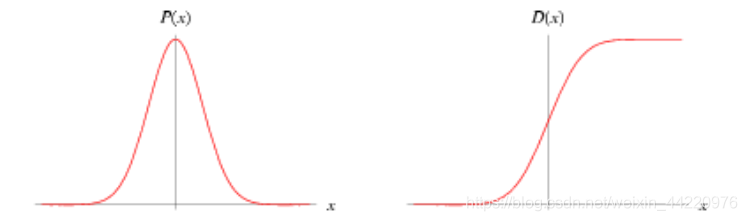
\includegraphics[scale=0.45]{imgs/chapter2/1}
\par\end{centering}
\caption{正态分布\protect\label{fig:2.1}}

\end{figure}

\begin{figure}
\begin{centering}
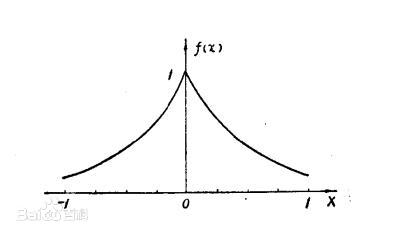
\includegraphics{imgs/chapter2/2}
\par\end{centering}
\caption{拉普拉斯分布\protect\label{fig:2.2}}

\end{figure}

\end{document}
